\subsection{Physical Architecture}
\label{sec:physical-architecture}

A physical architecture diagram shows all the hardware and software resources used by the application. This visual representation provides a clearer understanding of how these components communicate across the network. The physical architecture diagram is shown in Figure \ref{fig:physical-architecture-diagram}.

\begin{figure}[H]
    \centering
    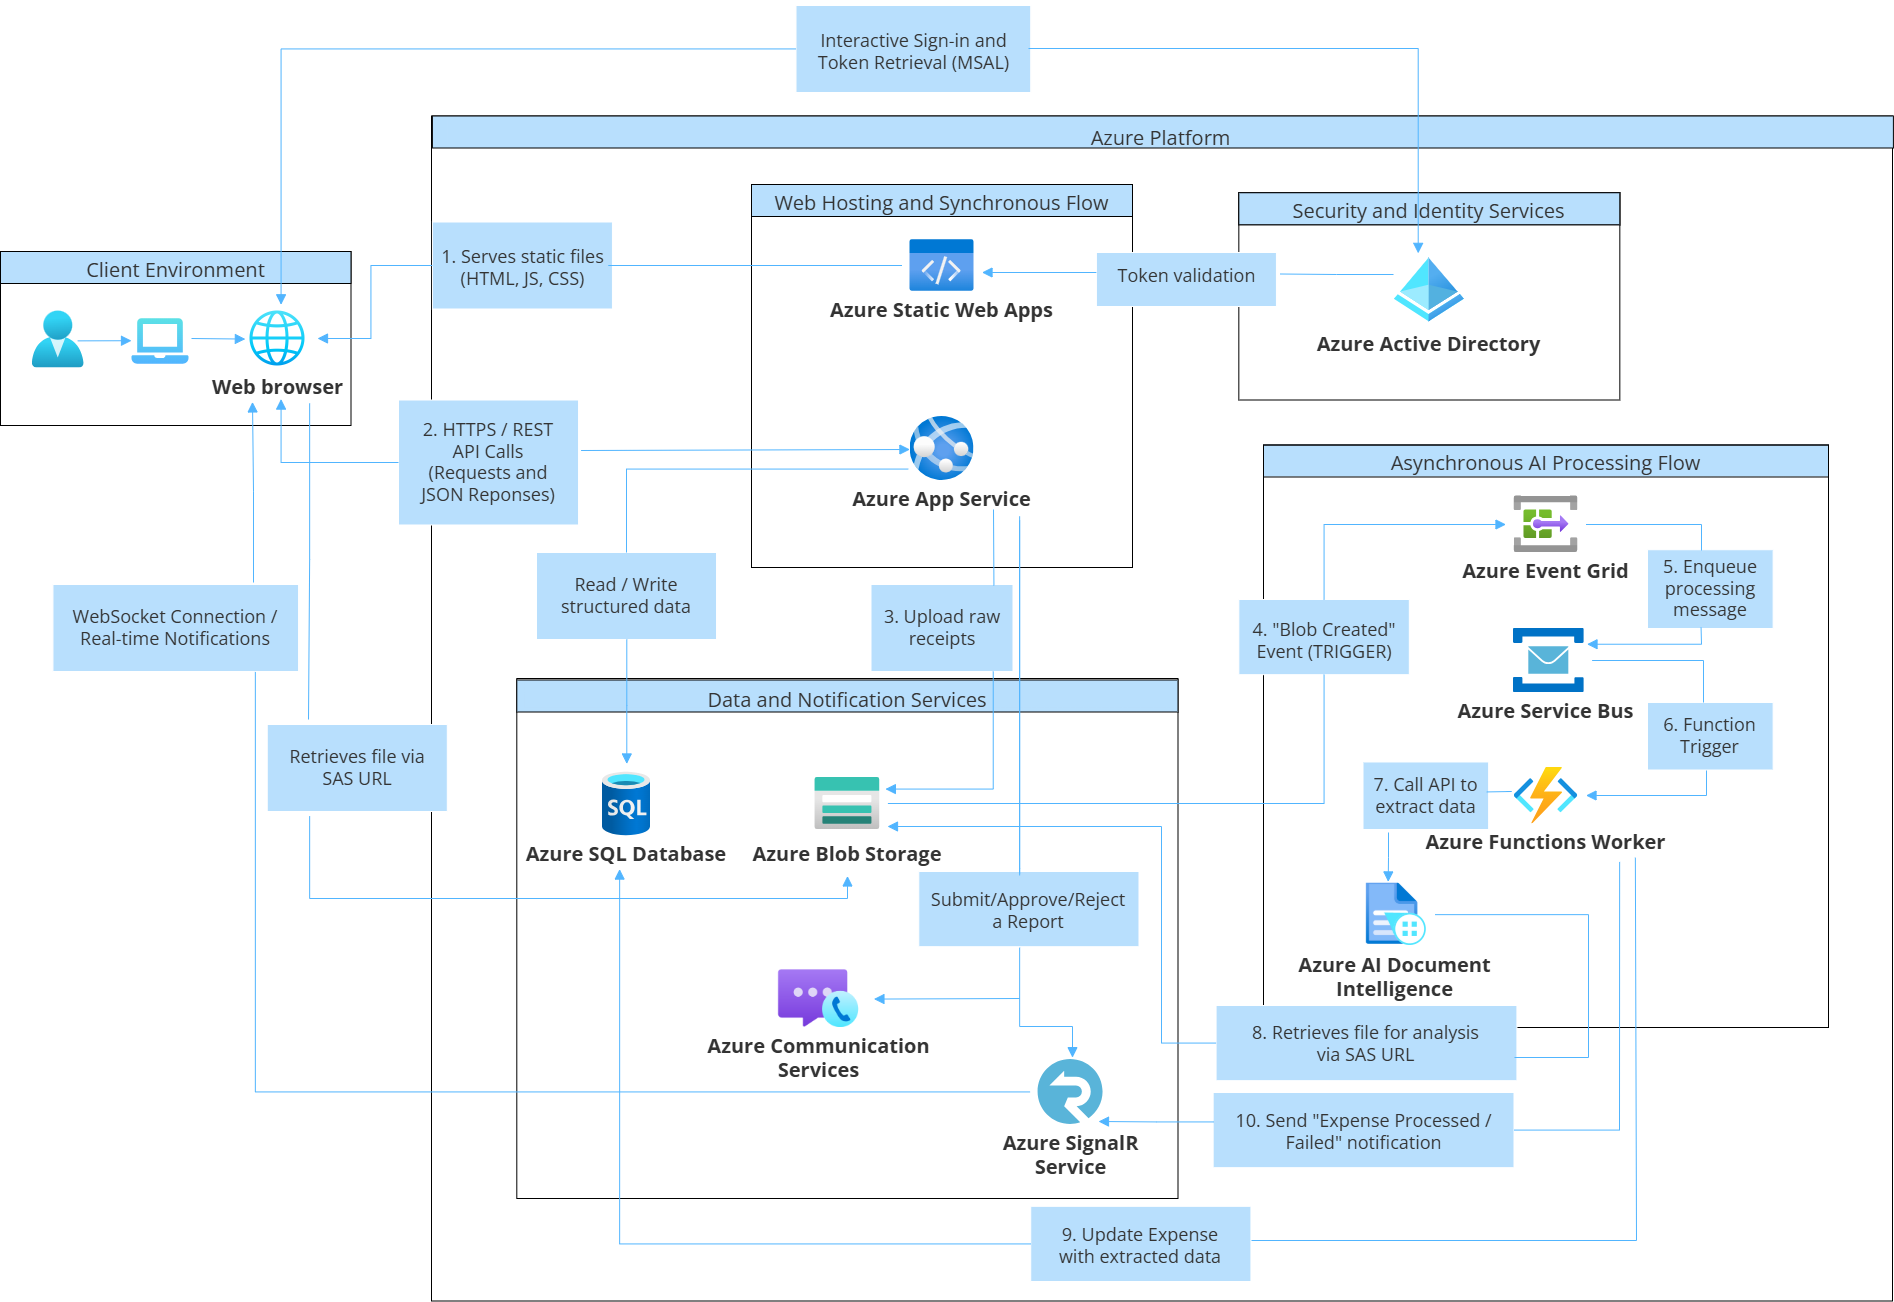
\includegraphics[width=\textwidth]{Images/PhysicalArchitecture.png}
    \caption[Physical architecture diagram]
    {Physical architecture diagram. [Own creation]}
    \label{fig:physical-architecture-diagram}
\end{figure}

The application's physical architecture follows a modern, cloud-native approach, leveraging Microsoft Azure Platform-as-a-Service (PaaS). It is structured around two main operational flows: the Synchronous Flow, which handles immediate user requests, and the Asynchronous AI Processing Flow, which executes complex tasks in the background. This design ensures scalability while maintaining a highly responsive user experience.

\vspace{0.5cm}

\textbf{The Client Environment and Synchronous Flow}

As defined in sub-objective SO2 in Section \ref{sec:objectives}, this project aims to develop a full-stack web application; consequently, the application comprises a frontend and a backend. The frontend is implemented as a React application and deployed using \textbf{Azure Static Web Apps}, while the backend is a .NET solution hosted on \textbf{Azure App Service}.

User interaction begins in the \textbf{Client Environment}, where the \textbf{web browser} executes the React application. Unlike traditional frontend architectures, where the React application communicates directly with the backend API, Azure Static Web Apps does not act as an intermediary in this interaction. Instead, the browser communicates directly with the backend service.

The interaction flow is as follows:

\begin{enumerate} [leftmargin=0.75cm, noitemsep]
    \item The user opens a \textbf{web browser} and navigates to the application URL.
    \item \textbf{Azure Static Web Apps} delivers the static assets (HTML, CSS, and JavaScript) with low latency via a Content Delivery Network (CDN).
    \item The application is executed locally in the user's browser, not on Azure Static Web Apps.
    \item The browser is responsible for making REST API requests to the backend.
\end{enumerate}

In this setup, \textbf{Azure Static Web Apps} serves only as a static content host. The benefit of this approach is that fast global access is accomplished, as assets are distributed through a CDN, reducing load times for users regardless of location. 

Consequently, as illustrated in Figure \ref{fig:physical-architecture-diagram}, the browser communicates directly with the backend hosted on \textbf{Azure App Service}.  This communication follows a standard HTTPS request-response pattern, represented as a bidirectional interaction (arrow). Each time the browser sends a request (e.g., upload a new expense or retrieve expense data), the API returns a JSON-formatted response. 

\textbf{Azure App Service} executes the .NET API and synchronously handles business logic, data validation, authentication, and authorization. Additionally, Azure App Service is also responsible for interacting with \textbf{data persistence and notification services}.

\vspace{0.5cm}

\textbf{Data Persistence}

The application uses two data storage services to support distinct storage approaches. \textbf{Azure SQL Database} is designed to persistently store structured, relational data, such as user information, expense metadata, and report details. In contrast, \textbf{Azure Blob Storage} is optimized for storing and retrieving large unstructured objects, specifically raw receipt files (binary files such as images and PDFs).

When the application needs to access previously uploaded receipt files, the browser interacts with \textbf{Azure Blob Storage}. A critical architectural pattern used here is the ``Valet Key Pattern'': each time the client requests a stored receipt, the backend API generates a temporary secure link, known as a Shared Access Signature (SAS) URL. Using this URL, the browser can securely download the file directly from \textbf{Azure Blob Storage}.

\vspace{0.5cm}

\textbf{The Asynchronous AI Processing Flow}

The Asynchronous Flow is an event-based solution designed to perform the heavy, complex task of extracting expense data using an AI model. At the same time, it avoids introducing significant delays that impact the user experience, preventing the user from having to wait until the expense is processed. This is achieved through an event-driven architecture, where the entire process is triggered whenever a new file is uploaded to the \textbf{Blob Storage}.

Once a file is uploaded, \textbf{Azure Event Grid}, a highly scalable service, immediately detects the ``Blob Created'' event and forwards the expense metadata. Instead of sending the expense directly to the AI for processing, it is queued to \textbf{Azure Service Bus}, a reliable container that acts as a durable buffer. In this way, if the processing service is temporarily unavailable, the request is not lost and will be handled once the service is recovered.

In response, the \textbf{Azure Function} is triggered when a new message is available in the Service Bus queue. The Function then orchestrates the analysis process: it first generates a temporary, secure access key (a SAS URL) for the newly uploaded receipt file stored in \textbf{Azure Blob Storage}. It then calls the \textbf{Azure AI Document Intelligence} service, providing this SAS URL.

Using the SAS URL, the Azure AI service directly and securely retrieves the receipt file from Blob Storage for processing and returns the extracted data in JSON format. The Azure Function receives the extracted data from the AI service and updates the corresponding expense record accordingly in Azure SQL Database. 

After successfully updating the database, the Function's final responsibility is to notify the user in real time. It sends a message to \textbf{Azure SignalR Service}, which instantly pushes a notification to the user's web browser, allowing the UI to update automatically and reflect that the expense has been processed. This event-driven design fully decouples the initial user action from the complex background workflow.

\vspace{0.5cm}

\textbf{Real-time Notifications}

Receiving real-time feedback is a key positive aspect of the user experience. Once the AI has finished processing the receipt, a message is sent to the \textbf{Azure SignalR Service}, which maintains a persistent WebSocket connection with the user's browser. 

Whenever the SinalR receives a “Expense Processed” message, it immediately pushes this notification to the client application. This approach allows the user to visualize a real-time update of the expense processing status without needing a manual page refresh. Moreover, \textbf{Azure Communication Services} dispatches email notifications to the interested user whenever a report is submitted or reviewed.

\vspace{0.5cm}

\textbf{Security and Identity Management}

The application's security is built upon \textbf{Azure Active Directory (Azure AD)}. Azure AD is an identity management system that acts as a central \textbf{Identity Provider (IdP)}. It not only handles user authentication but also serves as the authority for token issuance. The architecture implements a modern OAuth 2.0 and OpenID Connect flow. OAuth 2.0 is used for authorization, allowing applications to access resources on behalf of a user without knowing their password, while OpenID Connect is used for authentication and provides information about the user's identity.

The client side handles user interaction for signing in to the application and uses the Microsoft Authentication Library (MSAL) for orchestrating login popups and redirects against Azure AD. After the user successfully logs in, MSAL obtains a JWT access token and stores it securely in session storage. The diagram illustrates a two-way communication between the \textbf{browser} and \textbf{Azure AD} during this process.

All further communication with the backend, including \textbf{REST API} calls and real-time \textbf{SignalR} connections, is secured using this JWT token. On the client side, the token is automatically added to the Authorization header as a Bearer token to communicate with the backend API. The backend API, hosted on \textbf{Azure App Service}, is protected using Microsoft.Identity.Web library. This middleware intercepts each incoming request, validates the JWT signature, claims (such as issuer and audience) against Azure AD's OpenID Connect metadata endpoints, and establishes the user identity.

This validation step is shown in the diagram as a one-way communication from the \textbf{App Service} to \textbf{Azure AD}. After successful validation, controllers and SignalR hubs enforce access control using the \texttt{[Authorize]} attribute. The application also maps the token's object identifier claim to a specific user, allowing it to perform authorized actions.




